\documentclass[tikz,border=3mm,multi=tikzpicture]{standalone}
\usepackage[utf8]{inputenc}
\usepackage[T1]{fontenc}
\usepackage{helvet}
\renewcommand{\familydefault}{\sfdefault}
\usepackage{tikz}
\usetikzlibrary{angles,quotes,calc,intersections}
\begin{document}

\tikzset{every node/.append style={font=\sffamily\small}}
% TikZ 1
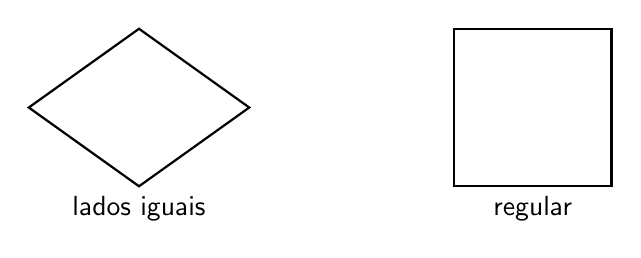
\begin{tikzpicture}[scale=1]
\draw[thick] (0,0)--(1.4,1)--(0,2)--(-1.4,1)--cycle;
\node[below] at (0,0) {lados iguais};
\draw[thick] (4,0) rectangle (6,2);
\node[below] at (5,0) {regular};
\end{tikzpicture}
% TikZ 2
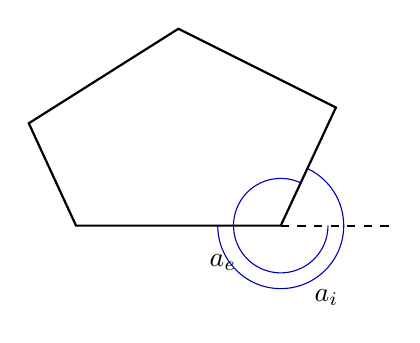
\begin{tikzpicture}[scale=1]
\coordinate (A) at (0,0); \coordinate (B) at (2.6,0); \coordinate (C) at (3.3,1.5); \coordinate (D) at (1.3,2.5); \coordinate (E) at (-.6,1.3); \coordinate (X) at (4,0);
\draw[thick] (A)--(B)--(C)--(D)--(E)--cycle;
\draw[thick,dashed] (B)--(X);
\pic[draw=blue!70!black, "$a_i$", angle radius=8mm, angle eccentricity=1.35] {angle=A--B--C};
\pic[draw=blue!70!black, "$a_e$", angle radius=6mm, angle eccentricity=1.45] {angle=C--B--X};
\end{tikzpicture}


% TikZ 3
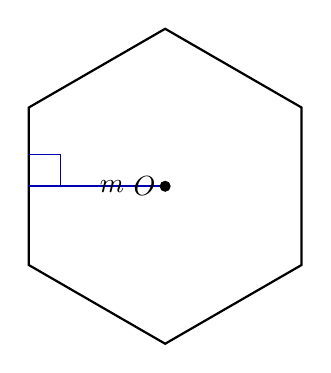
\begin{tikzpicture}[scale=1]
\coordinate (O) at (0,0);
\foreach \k in {1,...,6}{\coordinate (P\k) at ({90+60*(\k-1)}:2);}
\draw[thick] (P1)--(P2)--(P3)--(P4)--(P5)--(P6)--cycle;
\coordinate (M) at ($(P2)!0.5!(P3)$);
\draw[blue!70!black,thick] (O)--(M);
\pic[draw=blue!70!black, angle radius=4mm] {right angle=O--M--P2};
\fill (O) circle (2pt);
\node[left] at (O) {$O$};
\node[right] at ($(O)!0.55!(M)$) {$m$};
\end{tikzpicture}
% TikZ 4
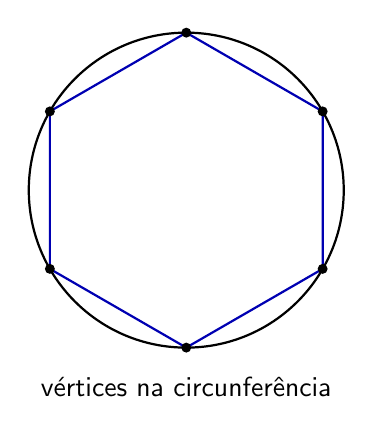
\begin{tikzpicture}[scale=1]
\coordinate (O) at (0,0);
\draw[thick] (O) circle (2);
\foreach \k in {1,...,6}{\coordinate (P\k) at ({90+60*(\k-1)}:2);}
\draw[thick,blue!70!black] (P1)--(P2)--(P3)--(P4)--(P5)--(P6)--cycle;
\foreach \k in {1,...,6}{\fill (P\k) circle (1.8pt);}
\node[below] at (0,-2.25) {vértices na circunferência};
\end{tikzpicture}


% TikZ 5
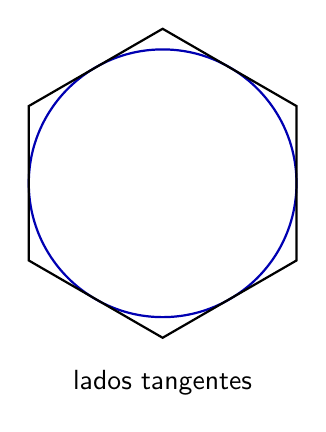
\begin{tikzpicture}[scale=1]
\coordinate (O) at (0,0);
\draw[thick,blue!70!black] (O) circle (1.7);
\foreach \k in {1,...,6}{\coordinate (P\k) at ({90+60*(\k-1)}:1.962);}
\draw[thick] (P1)--(P2)--(P3)--(P4)--(P5)--(P6)--cycle;
\node[below] at (0,-2.25) {lados tangentes};
\end{tikzpicture}
\end{document}
